\documentclass[]{article}
\usepackage{graphicx}
\usepackage{pgfplots}
\pgfplotsset{width=10cm,compat=1.9}
% We will externalize the figures
%\usepgfplotslibrary{external}
%\tikzexternalize
\pgfplotsset{
  every axis plot/.append style={line width=4pt},
  every axis plot post/.append style={
    every mark/.append style={line width=0.8pt}
  }
}
\usepackage{hyperref}
\hypersetup{
    colorlinks,
    linkcolor={blue!50!black},
    citecolor={blue!50!black},
    urlcolor={blue!80!black}
}
\usepackage{listings}
\usepackage{xcolor}



\definecolor{codegreen}{rgb}{0,0.6,0}
\definecolor{codegray}{rgb}{0.5,0.5,0.5}
\definecolor{sviolet}{HTML}{6C71C4}
\definecolor{codepurple}{rgb}{0.58,0,0.82}
\definecolor{backcolour}{rgb}{0.95,0.95,0.92}
\definecolor{sblue}{HTML}{268BD2}

\lstdefinestyle{formal}{
    backgroundcolor=\color{backcolour},   
    commentstyle=\color{codegreen},
    keywordstyle=\color{blue},
    numberstyle=\tiny\color{codegray},
    stringstyle=\color{sviolet},
    basicstyle=\ttfamily\footnotesize,
    breakatwhitespace=false,         
    breaklines=true,                 
    captionpos=b,                    
    keepspaces=true,                 
    numbers=left,                    
    numbersep=5pt,                  
    showspaces=false,                
    showstringspaces=false,
    showtabs=false,                  
    tabsize=2
}

\lstset{style=formal}

\usepackage{geometry}
    \geometry{
    a4paper,
    inner=3.75cm,
    outer=1.75cm,
    top=3cm,
    bottom=3.5cm,
    headheight=1.5cm,
    footskip=42pt}

\title{NSAE: Classroom problem 1.1}
\author{Miquel Borrell}
\date{}

\begin{document}

\maketitle

This document aims to solve the first Problem of the course. The statement is as follows:

\begin{figure}[h]
	\includegraphics[width=\textwidth]{Problem.png}
	\caption{Problem NSAE 1.1}
\end{figure}

First we will discuss the analytical solution and it will be followed by an coded solution.

\section{Analytical solution}

Let's take a look to the data on a graph (Figure \ref{fig:data_points_graph}):
\begin{figure}[h]
    \centering
    \begin{tikzpicture}[scale=1]
	\begin{axis}[
    	    xlabel={t(s)},
    	    ylabel={x(km)},
    	    xmin=0, xmax=3.5,
    	    ymin=0, ymax=1.2,
    	    legend pos=south east,
    	    ymajorgrids=true,
    	    grid style=dashed,
    	]
    	
    	\addplot[
    	    color=red,
    	    only marks,
    	    mark=*,
    	    ]
    	    coordinates{(0,0)(1,0.63)(2,0.86)(3,0.95)};
    	    \legend{data}
    	\end{axis}
    \end{tikzpicture}

   \caption{Data visualization}
   \label{fig:data_points_graph}
\end{figure}

Following the procedure explained in class we can calculate the polynomial between $t_0$ and $t_1$ using expression 29 and 35.
In this way we can find the coefficients of $p_{0,1}$ :

\begin{equation}
    P_{j,j+1}(t)=f_j + \left[ \frac{f_{j+1}-f_j}{h_j}-\frac{h_jp''_{j+1}}{6}-\frac{h_jp''_j}{3} \right] (t-t_j)+\frac{p''_j}{2}(t-t_j)^2+\frac{p''_{j+1}-p''_j}{6h_j}(t-t_j)^3
\end{equation}

In our case $p_{0,1}$ would be calculated as:

\begin{equation}\label{eq:p01}
    p_{0,1}=0+ \left[ \frac{0.63-0}{1}-\frac{1*p''_1}{6}-\frac{1*p''_0}{3} \right](t-0)+\frac{p''_0}{2}(t-0)^2+\frac{p''_1-p''_0}{6*1}(t-0)^3
\end{equation}

At this point we realize we need to calculate $p''_0$ and $p''_1$. But as we are working with natural splines $p''_0=0$. So in order to get $p''_1$ we will make use of expression 35 in the bibliography which states that:

\begin{equation}
    2(h_0+h_1)p''_1+h_1p''_2=\frac{6(x_2-x_1)}{h_1}-\frac{6(x_1-x_0)}{h_0}
\end{equation}
\begin{equation}
    h_1p''_1+2(h_1+h_2)p''_2+h_3p''_3=\frac{6(x_3-x_2)}{h_2}-\frac{x_2-x_1}{h_1}
\end{equation}

Where $h_j=(t_{j+1}-t_j)$ in this case $h_0=h_1=h_2=1$. Resolving we have:

\begin{equation}
    2(2)p''_1+p''_2=6(0.86-0.63)-6(0.63-0)
\end{equation}
\begin{equation}
    p''_1+4p''_2+p''_3=6(0.95-0.86)-(0.86-0.63)
\end{equation}

It results in:\[p''_1=-0.584\]\[p''_2=-0.064\]
This coupled with the natural splines condition means that we can now fully resolve equation \ref{eq:p01} and discover the best fitting cubic spline between $t_0$ and $t_1$:
\[p_{0,1}=0.7273t-0.0973t^3\] with coefficients being:
\[a_0=0.097\overline{3}\]
\[b_0=0\]
\[c_0=0.0727\overline{3}\]
\[d_0=0\]

Now let's look at the output of this polynomial in our case (Figure \ref{fig:p01_visualitzation}):
\begin{figure}[h]
    \centering
    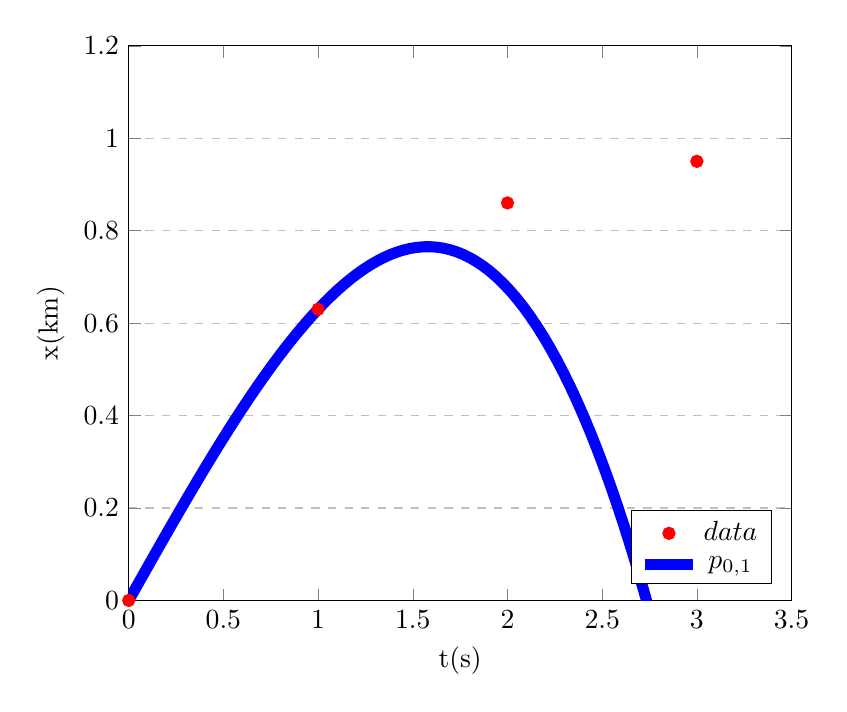
\begin{tikzpicture}[scale=1]
	\begin{axis}[
    	    xlabel={t(s)},
    	    ylabel={x(km)},
    	    xmin=0, xmax=3.5,
    	    ymin=0, ymax=1.2,
    	    legend pos=south east,
    	    ymajorgrids=true,
    	    grid style=dashed,
    	]
    	
    	\addplot[
    	    color=red,
    	    only marks,
    	    mark=*,
    	    ]
    	    coordinates{(0,0)(1,0.63)(2,0.86)(3,0.95)};
    	    \addlegendentry{\(data\)}
	\addplot[
	    domain=0:3.5, 
            samples=100, 
            color=blue,
            ]
	    {0.7273*x-0.0973*x^3};
	    \addlegendentry{\(p_{0,1}\)}
    	\end{axis}
    \end{tikzpicture}

   \caption{Data visualization}
   \label{fig:p01_visualitzation}
\end{figure}

We can observe that the cubic spline fits perfectly between the interval $0<=t<=1$.

Now we could repeat the process for the other points until we have a set of 3 polynomials for each data intervals. However we could also automate this using Python and the package Scipy which provides a handy way of computing all the coefficients and providing the polynomials. 
We could follow the code below:
\begin{lstlisting}[language=Python]
    import numpy as np
    import math
    from scipy import interpolate
    t=np.linspace(0,3,4,dtype=int)
    x=np.array([0,0.63,0.86,0.95])

    # calculate Cubic Spline using Scipy method
    cs=interpolate.CubicSpline(t,xd,bc_type='natural')
    
    #Print cs coeficients to construct polynomials (.T to transpose for easy visualitzation)
    print(cs.c.T)
        
\end{lstlisting}

The output of this code will produce is something like this:

\begin{lstlisting}[language=Python]
array([[-9.73333333e-02, -1.11022302e-16,  7.27333333e-01,
         0.00000000e+00],
       [ 8.66666667e-02, -2.92000000e-01,  4.35333333e-01,
         6.30000000e-01],
       [ 1.06666667e-02, -3.20000000e-02,  1.11333333e-01,
         8.60000000e-01]])
\end{lstlisting}

Which in turn can be interpreted as the following table:

\begin{table}[h]
\begin{tabular}{lllll}
           & a         & b         & c        & d        \\
$p_{0,1}$ & -9.73e-02 & -1.11e-16 & 7.27e-01 & 0.00e+00 \\
$p_{1,2}$ & 8.66e-02  & -2.92e-01 & 4.35e-01 & 6.30e-01 \\
$p_{2,3}$ & 1.06e-02  & -3.20e-02 & 1.11e-01 & 8.60e-01
\end{tabular}
\end{table}

Which translates to the following cubic splines:

\[p_{0,1}=0.7273t-0.0973t^3\]
\[p_{1,2}=0.0866(t-1)^3-0.292(t-1)^2+0.435(t-1)+0.630\]
\[p_{2,3}=0.0106(t-2)^3-0.032(t-2)^2+0.111(t-2)+0.860\]

Visually it would be translated to the following graph (Figure \ref{fig:cubic_splines_visualitzation}):

\begin{figure}[h]
    \centering
    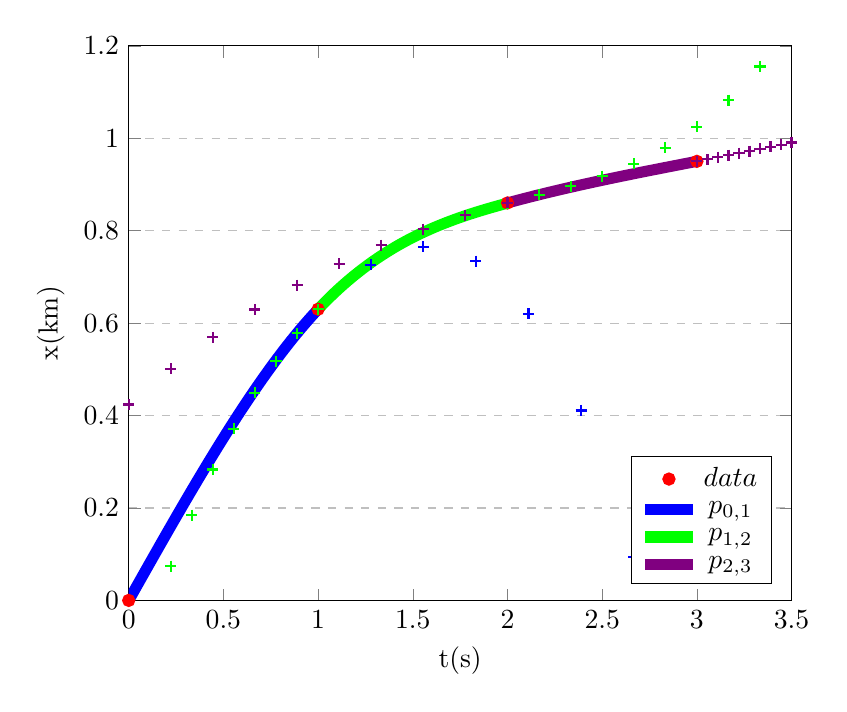
\begin{tikzpicture}[scale=1]
	\begin{axis}[
    	    xlabel={t(s)},
    	    ylabel={x(km)},
    	    xmin=0, xmax=3.5,
    	    ymin=0, ymax=1.2,
    	    legend pos=south east,
    	    ymajorgrids=true,
    	    grid style=dashed,
    	]
    	
    	\addplot[
    	    color=red,
    	    only marks,
    	    mark=*,
    	    ]
    	    coordinates{(0,0)(1,0.63)(2,0.86)(3,0.95)};
    	    \addlegendentry{\(data\)}
	\addplot[
	    domain=0:1, 
            samples=100, 
            color=blue,
	    ]
	    {0.7273*x-0.0973*x^3};
	    \addlegendentry{\(p_{0,1}\)}
	
	\addplot[
	    forget plot,
	    domain=1:3.5, 
            samples=10, 
            color=blue,
	    mark=+,
	    only marks,
            ]
	    {0.7273*x-0.0973*x^3};
	
	\addplot[
	    domain=1:2, 
            samples=100, 
            color=green,
            ]
	    {0.0866*(x-1)^3-0.292*(x-1)^2+0.435*(x-1)+0.630};
	    \addlegendentry{\(p_{1,2}\)}
	\addplot[
	    forget plot,
	    domain=0:1, 
            samples=10, 
            color=green,
	    mark=+,
	    only marks,
            ]
	    {0.0866*(x-1)^3-0.292*(x-1)^2+0.435*(x-1)+0.630};
	\addplot[
	    forget plot,
	    domain=2:3.5, 
            samples=10, 
            color=green,
	    mark=+,
	    only marks,
            ]
	    {0.0866*(x-1)^3-0.292*(x-1)^2+0.435*(x-1)+0.630};
	\addplot[
	    forget plot,
	    domain=0:2, 
            samples=10, 
            color=violet,
	    mark=+,
	    only marks,
            ]
	    {0.01066667*(x-2)^3-0.032*(x-2)^2+0.11133333*(x-2)+0.86};
	 \addplot[
	    domain=2:3, 
            samples=100, 
            color=violet,
            ]
	    {0.01066667*(x-2)^3-0.032*(x-2)^2+0.11133333*(x-2)+0.86};
	    \addlegendentry{\(p_{2,3}\)}
	\addplot[
	    forget plot,
	    domain=3:3.5, 
            samples=10, 
            color=violet,
	    mark=+,
	    only marks,
            ]
	    {0.01066667*(x-2)^3-0.032*(x-2)^2+0.11133333*(x-2)+0.86};

    	\end{axis}
    \end{tikzpicture}

   \caption{Representation of the splines}
   \label{fig:cubic_splines_visualitzation}
\end{figure}

Furthermore we can compare the result with the analytical solution to grasp a sense of the error committed by this approximation as we can see in the figure \ref{fig:spline_vs_analytical}:

\begin{figure}[h]
    \centering
    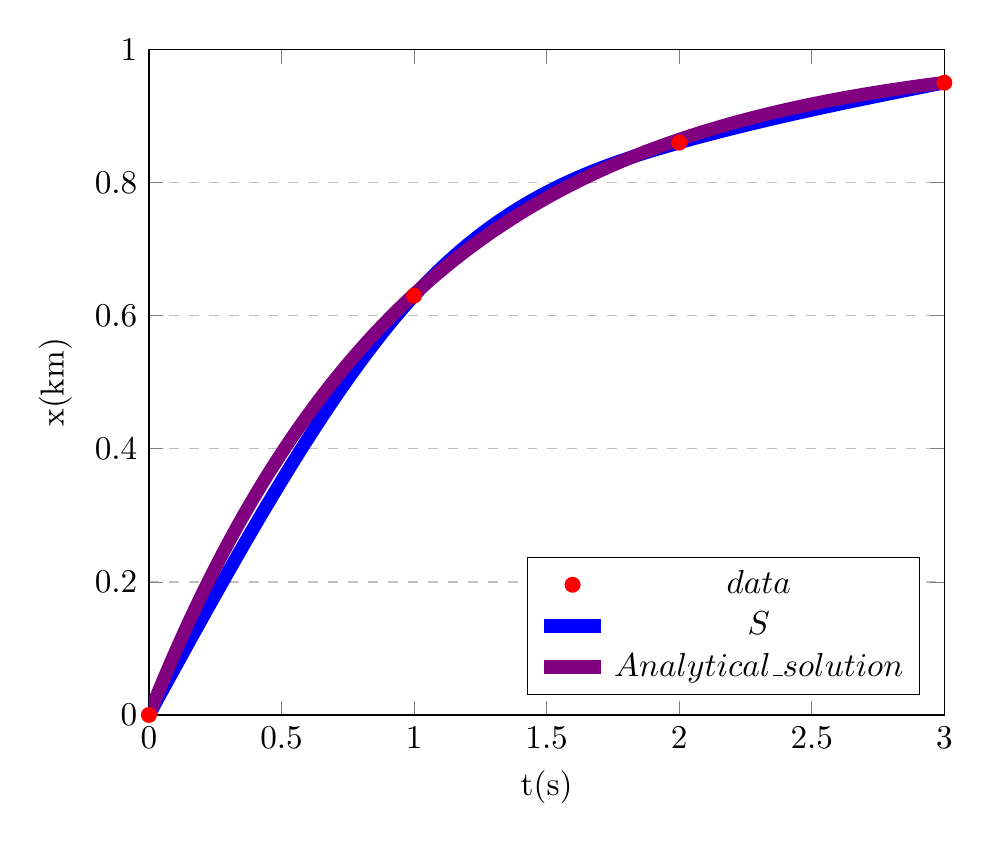
\begin{tikzpicture}[scale=1.2]
	\begin{axis}[
    	    xlabel={t(s)},
    	    ylabel={x(km)},
    	    xmin=0, xmax=3,
    	    ymin=0, ymax=1,
    	    legend pos=south east,
    	    ymajorgrids=true,
    	    grid style=dashed,
    	]
    	
    	\addplot[
    	    color=red,
    	    only marks,
    	    mark=*,
    	    ]
    	    coordinates{(0,0)(1,0.63)(2,0.86)(3,0.95)};
    	    \addlegendentry{\(data\)}
	\addplot[
	    domain=0:1, 
            samples=100, 
            color=blue,
	    ]
	    {0.7273*x-0.0973*x^3};
	    \addlegendentry{\(S\)}
	
	\addplot[
	    forget plot,
	    domain=1:2, 
            samples=100, 
            color=blue,
            ]
	    {0.0866*(x-1)^3-0.292*(x-1)^2+0.435*(x-1)+0.630};
	\addplot[
	    forget plot,
	    domain=2:3, 
            samples=100, 
            color=blue,
            ]
	    {0.01066667*(x-2)^3-0.032*(x-2)^2+0.11133333*(x-2)+0.86};
	\addplot[
	    domain=0:3, 
            samples=100, 
            color=violet,
            ]
	    {(1-exp(-x))};
	    \addlegendentry{\(Analytical\_solution\)}
    	\end{axis}
    \end{tikzpicture}

   \caption{Comparison between analytical and approximation solutions}
   \label{fig:spline_vs_analytical}
\end{figure}


Going one step further we can also take a look to the derivatives of our splines in figure \ref{fig:spline_drivatives}

\begin{figure}[h]
    \centering
    \includegraphics[width=1.1\textwidth]{Splines_derivatives.png}
    \caption{Spline derivatives}
    \label{fig:spline_drivatives}
\end{figure}

We can observe the continuity of the derivative up to the third derivation.
\end{document}
